\documentclass[
	% -- opções da classe memoir --
	12pt,				% tamanho da fonte
	openright,			% capítulos começam em pág ímpar (página vazia se preciso)
% 	twoside,			% para impressão em recto e verso.
    oneside,
	a4paper,			% tamanho do papel. 
	% -- opções da classe abntex2 --
	chapter=TITLE,
% 	section=Title,
% 	subsection=Title,
% 	subsubsection=Title,
	% -- opções do pacote babel --
	english,			% idioma adicional para hifenização
% 	french,				% idioma adicional para hifenização
% 	spanish,			% idioma adicional para hifenização
	brazil				% o último idioma é o principal do documento
	]{./abntex2}

% ---
% Pacotes básicos 
% ---
\usepackage{lmodern}		% Usa a fonte Latin Modern	
\usepackage{float}
\usepackage[T1]{fontenc}	% Selecao de codigos de fonte.
\usepackage[utf8]{inputenc}	% Codificacao do documento 
\usepackage{indentfirst}	% Indenta o primeiro parágrafo de cada seção.
\usepackage{color}			% Controle das cores
\usepackage{graphicx}		% Inclusão de gráficos
\usepackage{microtype} 		% para melhorias de justificação
\usepackage{setspace}       % para espacamento simples no resumo
\usepackage{pdfpages}
% ---
		
% ---
% Pacotes adicionais, usados apenas no exemplo
% ---
\usepackage{lipsum} % para geração de dummy text
% ---

% ---
% Pacotes de citações
% ---
%\usepackage[brazilian,hyperpageref]{backref} % Mostra a página onde cada citação foi feita
\usepackage[alf,abnt-etal-list=0,bibjustif]{./abntex2cite} % Citações numéricas (ordem de apresentação)
%\usepackage[alf,abnt-etal-list=0,bibjustif]{./abntex2cite} % Citações autor-data (ordem alfabética)

% --- 
% CONFIGURAÇÕES DE PACOTES
% --- 
%Adicionados pelo Maj Maurício
%referência cruzada com página
\newcommand{\cref}[1]{\ref{#1} (pág. \pageref{#1})}
%citação autor (ano).
\newcommand{\citep}[1]{\citeauthor{#1} (\citeyear{#1})}

% % ---
% % Configurações do pacote backref, SE FOR USAR DESCOMENTE TODO ESSE TRECHO
% % Usado sem a opção hyperpageref de backref
% \renewcommand{\backrefpagesname}{Citado na(s) página(s):~}
% % Texto padrão antes do número das páginas
% \renewcommand{\backref}{}
% % Define os textos da citação
% \renewcommand*{\backrefalt}[4]{
% 	\ifcase #1 %
% 		Nenhuma citação no texto.%
% 	\or
% 		Citado na página #2.%
% 	\else
% 		Citado #1 vezes nas páginas #2.%
% 	\fi}%
% % ---


% ---
% Informações de dados para CAPA e FOLHA DE ROSTO
% ---
\usepackage{abntex2ime}
% ---



% ---
% EXEMPLO PARA CURSO DE POS GRADUAÇÃO
% ---

% \instituicao{Instituto Militar de Engenharia}
% \programapgdepartamento{Engenharia de Transportes}
% \nivelestudo{Doutorado} % Graduação, Mestrado ou Doutorado
% % ---
% \titulo{Modelo Canônico de Trabalho Acadêmico com \abnTeX\space \versaoDocumento}
% \palavraschave{arp,sarp,iot,vant,tarefas cooperativas,agentes inteligentes}
% \keywords{unmanned systems,unmanned vehicles,uav,uas,cooperative tasks,intelligent agents}
% % ---
% \autores{Fulano de}{Silva}% 1+ autores
% % \autor{Fulano de}{Tal} %{nome}{sobrenome}
% \orientadores{Sicrano,Beltrano}{Santos,Oliveira}{Ph.D.,D.Sc.}%{nomes}{sobrenomes}{títulos}
% % ---
% \local{Rio de Janeiro}
% \data{2020}
% \datadefesa{30 de fevereiro de 2020}
% \bancadeexaminadores{
%     Prof. \textbf{Orientador 1} - D.Sc. do IME - Presidente,
%     Prof. \textbf{Orientador 2} - D.Sc. do LNCC,
%     Prof. \textbf{Professor 1} - Ph.D. do IMPA,
%     Prof. \textbf{Professor 2} - D.Sc. do LNCC,
%     Prof. \textbf{Professor 3} - D.Sc. do IME,
%     Prof. \textbf{Professor 4} - D.Sc. da PUC
% }

% ---



% ---
% EXEMPLO PARA PROJETO DE FIM DE CURSO
% ---

\instituicao{Instituto Militar de Engenharia}
\programapgdepartamento{Engenharia Cartográfica}
\nivelestudo{Graduação} % Graduação, Mestrado ou Doutorado
% ---
\titulo{Modelo Canônico de Trabalho Acadêmico com \abnTeX\space \versaoDocumento}
\palavraschave{arp,sarp,iot,vant,tarefas cooperativas,agentes inteligentes}
\keywords{unmanned systems,unmanned vehicles,uav,uas,cooperative tasks,intelligent agents}
% ---
\autores{Fulano da,Ciclano}{Silva,Pereira}% {nome}{sobrenome} 1+
\orientadores{Sicrano,Beltrano}{Santos,Oliveira}{Ph.D.,D.Sc.}%{nomes}{sobrenomes}{títulos} 1+
% ---
\local{Rio de Janeiro}
\data{2025}
\datadefesa{10 de Outubro de 2024}
\bancadeexaminadores{
    \textbf{Maj Maurício Carvalho Mathias de Paulo - D.Sc do IME},
    \textbf{Cel Marcos de Meneses Rocha - D.Sc do IME},
    \textbf{Maj Felipe Ferrari - D.E do IME},
    \textbf{TC Ivanildo Barbosa - D.Sc do IME} 
}

% ---



% ---
% Configurações de aparência do PDF final

% % alterando o aspecto da cor azul
% \definecolor{blue}{RGB}{41,5,195}

% % informações do PDF
\makeatletter
\hypersetup{
    %pagebackref=true,
    % pdftitle={\@title}, 
    % pdfauthor={\@author},
    % pdfsubject={\imprimirpreambulo},
    % pdfcreator={LaTeX with abnTeX2},
    colorlinks=true, % false: boxed links; true: colored links
    linkcolor=black, % color of internal links
    citecolor=black,	% color of links to bibliography
    filecolor=black, % color of file links
    urlcolor=black,
    bookmarksdepth=4
}
\makeatother
% % --- 
% % --- 

% ---
% Posiciona figuras e tabelas no topo da página quando adicionadas sozinhas
% em um página em branco. Ver https://github.com/abntex/abntex2/issues/170
\makeatletter
\setlength{\@fptop}{5pt} % Set distance from top of page to first float
\makeatother
% ---

% ---
% Possibilita criação de Quadros e Lista de quadros.
% Ver https://github.com/abntex/abntex2/issues/176
%
\newcommand{\quadroname}{Quadro}
\newcommand{\listofquadrosname}{Lista de quadros}

%\newfloat[chapter]{quadro}{loq}{\quadroname}
\newlistof{listofquadros}{loq}{\listofquadrosname}
\newlistentry{quadro}{loq}{0}

% configurações para atender às regras da ABNT
\setfloatadjustment{quadro}{\centering}
\counterwithout{quadro}{chapter}
\renewcommand{\cftquadroname}{\quadroname\space} 
\renewcommand*{\cftquadroaftersnum}{\hfill--\hfill}

\setfloatlocations{quadro}{hbtp} % Ver https://github.com/abntex/abntex2/issues/176
% ---

% --- 
% Espaçamentos entre linhas e parágrafos 
% --- 

% O tamanho do parágrafo é dado por:
\setlength{\parindent}{1.3cm}

% Controle do espaçamento entre um parágrafo e outro:
\setlength{\parskip}{0.2cm}  % tente também \onelineskip

% ---
% compila o indice
% ---
\makeindex
% ---

% ----
% Início do documento
% ----
\begin{document}

% Seleciona o idioma do documento (conforme pacotes do babel)
%\selectlanguage{english}
\selectlanguage{brazil}

% Retira espaço extra obsoleto entre as frases.
\frenchspacing 

% ----------------------------------------------------------
% ELEMENTOS PRÉ-TEXTUAIS
% ----------------------------------------------------------
% \pretextual

% ---
% Capa
% ---
\imprimircapa
% ---

% ---
% Folha de rosto
% (o * indica que haverá a ficha bibliográfica)
% ---
%\imprimirfolhaderosto*
% ---

% ---
% Inserir a ficha bibliografica
% ---

% \begin{fichacatalografica}
%     \includepdf{fig_ficha_catalografica.pdf}
% \end{fichacatalografica}

%\imprimirfichacatalografica
% ---

% ---ver
% Inserir folha de aprovação
% ---


\imprimirfolhadeaprovacao
% ---

% ---
% Dedicatória
% ---
%\begin{dedicatoria}
%   \vspace*{\fill}
%   \centering
%   \noindent
%   \textit{ Este trabalho é dedicado aos estudantes apaixonados que, apesar das dificuldades, nunca deixaram de acreditar no poder transformador do conhecimento.} \vspace*{\fill}
%\end{dedicatoria}
% ---

% ---
% Agradecimentos
% ---
\begin{agradecimentos}
Primeiramente, gostaríamos de agradecer às nossas famílias, que sempre estiveram
ao nosso lado, oferecendo amor, incentivo e apoio incondicional. Aos nossos pais, por serem fontes inesgotáveis de inspiração e por nos ensinarem a importância da perseverança.
Vocês são nossa base e nossa força.
Ao nossos orientadores Maj Maurício e Cel Marcos, pela orientação meticulosa, paciência e conhecimento compartilhado ao longo deste processo. Seus conselhos e críticas construtivas foram fundamentais para moldar este trabalho.
Aos amigos que estiveram ao nosso lado, nos motivaram e entenderam nossa ausência
em tantos momentos importantes. Seus sorrisos e palavras de encorajamento foram o
combustível que nos impulsionou.
Agradecemos também a todos os professores e funcionários da instituição, que contribuíram indiretamente para a nossa formação acadêmica.
Por último, mas não menos importante, agradecemos a todos aqueles que, de uma forma
ou de outra, nos apoiaram e encorajaram durante este percurso. Cada gesto de carinho,
cada palavra amiga e cada ato de gentileza foram fundamentais para nossa motivação e
bem-estar.
% \footnote{Os nomes dos integrantes do primeiro projeto abn\TeX\ foram extraídos de \url{http://codigolivre.org.br/projects/abntex/}}

Agradecimentos especiais são direcionados aos alunos da Engenharia Cartográfica 2024 que compartilharam conosco muitas noites de estudo, debates estimulantes e momentos de desafio e que contribuíram e que sempre irão contribuir para a manuntenção do conhecimento.

\end{agradecimentos}
% ---

% ---
% Epígrafe
% ---
%\begin{epigrafe}
%    \vspace*{\fill}
%	\begin{flushright}
%		\textit{``Conhecimento é a única riqueza que, \\
%                    quanto mais compartilhada, mais cresce.\\
%		(Provérbio Chinês)}
%	\end{flushright}
%\end{epigrafe}
% ---

% ---
% RESUMOS
% ---

% resumo em português
\setlength{\absparsep}{18pt} % ajusta o espaçamento dos parágrafos do resumo
\begin{resumo}
\SingleSpacing

% Motivação
% O que foi feito
% Quais resultados são esperados ou foram alcançados
% Breve fechamento dos principais impactos do que foi feito


 \textbf{Palavras-chave}: \imprimirpalavraschave
\end{resumo}

% resumo em inglês
\begin{resumo}[Abstract]
\begin{otherlanguage*}{english}
\linespread{1.3}
\SingleSpacing
% Usem o DeepL no resumo e corrijam.
This part will be written by the VF.

%This is the english abstract.
\vspace{\onelineskip}
\noindent 
\textbf{Keywords}: \imprimirkeywords
\end{otherlanguage*}
\end{resumo}

% ---
% inserir lista de ilustrações
% ---
%\pdfbookmark[0]{\listfigurename}{lof}
%\listoffigures*
%\cleardoublepage
% ---

% ---
% inserir lista de quadros
% ---
%\pdfbookmark[0]{\listofquadrosname}{loq}
%\listofquadros*
%\cleardoublepage
% ---

% ---
% inserir lista de tabelas
% ---
%\pdfbookmark[0]{\listtablename}{lot}
%\listoftables*
%\cleardoublepage
% ---

% ---
% inserir lista de abreviaturas e siglas
% ---
\begin{siglas} %ordem alfabética
  \item[CSW] Catalogue Service for the Web
  \item[HTTP] Hypertext Transfer Protocol
  \item[OGC] Open Geospatial Consortium
  \item[WCS] Web Coverage Service
  \item[WFS] Web Feature Service
  \item[WMS] Web Map Service
  \item[WMTS] Web Map Tile Service
  \item[MGB] Perfil de Metadados Geoespaciais do Brasil
  \item[REST] Representational State Transfer
  \item[JSON] JavaScript Object Notation
\end{siglas}
% ---

% ---
% inserir lista de símbolos
% ---
%\begin{simbolos}
%  \item[$ \Gamma $] Letra grega Gama
%  \item[$ \Lambda $] Lambda
%  \item[$ \zeta $] Letra grega minúscula zeta
%  \item[$ \in $] Pertence
%\end{simbolos}
% ---


% ---
% inserir o sumario
% ---

\makeatletter
\let\oldcontentsline\contentsline
\def\contentsline#1#2{%
    \oldcontentsline{#1}{\MakeTextUppercase{#2}}%
}
\makeatother

\pdfbookmark[0]{\contentsname}{toc}
\tableofcontents*
\cleardoublepage
% ---

% ----------------------------------------------------------
% ELEMENTOS TEXTUAIS
% ----------------------------------------------------------
\textual

% ----------------------------------------------------------
% Introdução (exemplo de capítulo sem numeração, mas presente no Sumário)
% ----------------------------------------------------------
\chapter{Introdução}
% ----------------------------------------------------------
\section{Justificativa do projeto}

% Contexto
% Problema a ser resolvido 

\section{Objetivo do projeto}

% Verificar com o orientador


\chapter{Fundamentação Teórica}
% Todo capítulo longo deve ser iniciado com um parágrafo que descreve o que será falado nesse capítulo, como uma visão geral. Tente explicar como isso se encaixa na compreensão geral do texto.

% Criar uma seção para cada tópico.
% Os tópicos devem contemplar o conteúdo que um engenheiro cartógrafo não conseguiria lembrar de cabeça e é necessário para a compreensão do trabalho de vocês. Devem ser evitadas explicações profundas e enfadonhas.

\chapter{Materiais e métodos}
% Todo capítulo longo deve ser iniciado com um parágrafo que descreve o que será falado nesse capítulo, como uma visão geral. Tente explicar como isso se encaixa na compreensão geral do texto.

%Este capítulo apresenta os materiais e métodos utilizados no desenvolvimento da aplicação. Serão abordados os requisitos, arquitetura da solução e ferramentas e tecnologias de desenvolvimento empregadas na solução final.

\section{Gestão do projeto}

\subsection{Partes interessadas}

As partes interessadas nesta aplicação são:
\begin{itemize} 
\item \textbf{DSG}: Espera um componente que tenha as mesmas funcionalidades do sistema atual, mas permita a evolução e integração com novos componentes.
\item \textbf{Chefes de Divisão de Geoinformação}: Autorizam a publicação de produtos. Gostariam que o sistema verificasse diferentes aspectos de qualidade dos produtos e metadados cadastrados, para auxiliar na decisão de publicar ou não.
\item \textbf{Cadastradores de metadados}: Vão inserir produtos no sistema. Desejam que o sistema tenha o máximo de automação para reduzir horas trabalhadas e aumentar a quantidade de produtos carregados por dia.
\item \textbf{Consumidores dos produtos cartográficos}: Desejam acessar e pesquisar produtos cartográficos na aplicação e também pelo servidor OGC CSW.
\end{itemize}

\subsection{Requisitos}
\label{sec:requisitos}

Os requisitos do sistema de cadastro de metadados foram organizados em duas categorias principais: requisitos funcionais, que descrevem as funcionalidades que a aplicação deve fornecer, e requisitos não funcionais, que especificam as qualidades que o sistema deve atender.

\subsection{Requisitos Funcionais}
\begin{itemize}
    \item \textbf{Cadastro otimizado de metadados}: Simplificar o processo de registro de informações pelos cadastradores de metadados, com a automatização da extração de dados dos arquivos geoespaciais e de metadados, bem como a possibilidade de realizar requisições diretamente ao servidor da aplicação.
    
    \item \textbf{Ferramentas para o gerenciamento dos metadados}: Prover ferramentas para a verificação da precisão e consistência dos metadados cadastrados, além de gerenciar todos os arquivos submetidos para assegurar a qualidade dos dados no BDGEx.
    
    \item \textbf{Criação de metadados no \textit{Front-end}}: Implementar uma interface que permita a criação de metadados, seguindo os padrões da ET-PCDG, para cada tipo de produto geoespacial.
    
    \item \textbf{Integração com o sistema CadastroGeral}: Consumir os dados gerais da produção cartográfica de cada CGeo por meio de uma API Rest para preenchimento automático de informações no sistema.
    
    \item \textbf{Importação de XML de metadados no \textit{Back-end}}: O sistema deve permitir a importação de arquivos XML contendo metadados já preenchidos, para simplificar o processo de cadastro.
    
    \item \textbf{Validação de XML de metadados no \textit{Back-end}}: Implementar validações automáticas dos arquivos XML de metadados, assegurando conformidade com as normas da ET-PCDG e da NT-CMet, para garantir a integridade dos dados.
\end{itemize}

\subsection{Requisitos Não Funcionais}
\begin{itemize}
    \item \textbf{Usabilidade}: O sistema deve proporcionar uma interface amigável e intuitiva para os operadores, facilitando o cadastro e a navegação entre os diferentes módulos da aplicação.
    
    \item \textbf{Desempenho}: O sistema deve ser capaz de processar grandes volumes de metadados (\textit{gigabytes}) de forma eficiente, garantindo tempos de resposta rápidos nas consultas e operações de importação/exportação de dados.

    \item \textbf{Integração com outros sistemas geoespaciais}: Desenvolver a aplicação para facilitar a integração com outras plataformas geoespaciais, conforme os padrões da OGC e das ISOs, possibilitando o intercâmbio de dados entre entidades.
    
   \item \textbf{Conformidade com padrões internacionais}: Garantir que o sistema esteja de acordo com os padrões ISO 19115 e ISO 19139 para metadados geoespaciais, além de atender às normativas do Exército Brasileiro, como a ET-PCDG e o MGB.
\end{itemize}


\newpage
\section{Escopo}

\subsection{Estrutura analítica do projeto (EAP)}
% Exemplo de site para produzir a EAP: https://editor.plantuml.com/uml/SoWkIImgAKygvj9I22ZApqejoUVIqb9mpIifIaq_lB0iDKV142YWfH2IM9IQbgY0n4PNPuGgXvtja9gN0h8D0000

% Quando vocês não tiverem ideia de tudo que precisa ser feito, usem o planejamento em ondas sucessivas. Ou seja, na VE vocês vão colocar na EAP os principais entregáveis e tarefas mais longas que vocês já sabem que precisam fazer. Na VC, é bom que vocês tenham já uma visão macro de todas as etapas que serão feitas. Na VF, vocês podem apresentar o que realmente aconteceu durante o trabalho.

% Se o projeto de vocês não for completamente preditivo, planejem um MVP (produto mínimo de valor), que é o mínimo necessário para que o projeto entregue algo de sucesso. Levantem funcionalidades opcionais, que serão acessórias, que podem ser contempladas no projeto (desejáveis, mas não obrigatórias). Após atingirem o MVP, introduzam estas funcionalidades para agregar valor ao trabalho. Todas as que foram pensadas e não foram contempladas, devem ser relatadas nos trabalhos futuros (conclusão).

\begin{figure}[H] % O [H] força a posição da figura
    \centering
    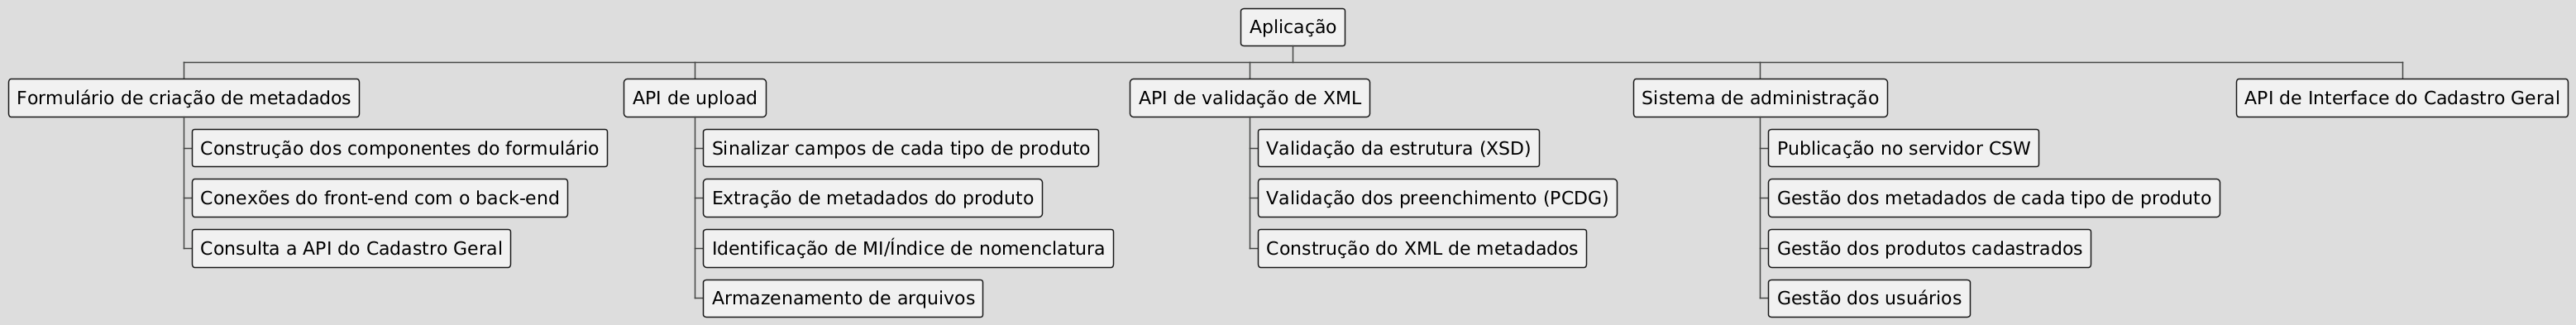
\includegraphics[width=1\linewidth, height=0.15\textheight]{img/EAP do projeto.png}
    \caption{Estrutura analítica do projeto.}
    \label{fig:eap} % Rótulo para referência cruzada
\end{figure}

\subsection{Dicionário da EAP}
% O ideal é que na EAP os itens estejam numerados utilizando a mesma numeração do Dicionário. No plantuml os números devem ser adicionados manualmente, então deixem para numerar no final (e não esqueçam, como aconteceu).
\begin{itemize}
   \item \textbf{1. Aplicação}
    \begin{itemize}
        \item \textbf{Descrição:} Projeto principal que abrange todas as atividades relacionadas à criação, desenvolvimento e administração da aplicação.
    \end{itemize}

    \item \textbf{1.1. Formulário de criação de metadados}
    \begin{itemize}
        \item \textbf{Descrição:} Desenvolvimento do \textit{front-end} responsável pela criação e gerenciamento do formulário de metadados.
        \item \textbf{Subcomponentes:}
        \begin{itemize}
            \item \textbf{1.1.1. Construção dos componentes:} Desenvolvimento dos componentes em React que serão parte integrante do formulário, como os campos do formulário e a tela de upload de arquivo.
            \item \textbf{1.1.2. Conexões do \textit{front-end} com o \textit{back-end}:} Conexões com as APIs do \textit{back-end} de tal forma a transformar o preenchimento do formulário dinâmico.
            \item \textbf{1.1.3. Consulta à API do Cadastro Geral:} Assegurar a responsividade às consultas a API REST que intermedia as informações para a obtenção de dados do sistema do Cadastro Geral.
        \end{itemize}
    \end{itemize}

    \item \textbf{1.2. API de upload}
    \begin{itemize}
        \item \textbf{Descrição:} API dedicada ao upload de metadados e produtos geoespaciais.
        \item \textbf{Subcomponentes:}
        \begin{itemize}
            \item \textbf{1.2.1. Sinalizar tipos de produtos:} Identificação dos tipos de produto a partir da extensão do arquivo.
            
            \item \textbf{1.2.2. Extração de metadados do produto:} Processo de extração de metadados a partir de um produto geoespacial.
            
            \item \textbf{1.2.3. Identificação de MI/Índice de nomenclatura:} Desenvolver um mecanismo de identificação e seleção automatizada do Índice de Nomenclatura a partir de produtos geoespaciais.
            
            \item \textbf{1.2.4. Armazenamento dos arquivos:} Estrutura de armazenamento para os arquivos de metadados e produtos geoespaciais.
        \end{itemize}
    \end{itemize}

    \item \textbf{1.3. API de validação de XML}
    \begin{itemize}
        \item \textbf{Descrição:} API que valida a estrutura e o conteúdo dos arquivos XML de metadados nos padrões nacionais e internacionais.
        \item \textbf{Subcomponentes:}
        \begin{itemize}
            \item \textbf{1.3.1. Validação da estrutura (XSD):} Verificação da conformidade dos XMLs com os esquemas XSD definidos para cada tipo de produto.
            \item \textbf{1.3.2. Validação dos preenchimentos (ET-PCDG):} Validação dos preenchimentos conforme os padrãos da ET-PCDG e NT-CMet.
            \item \textbf{1.3.3. Construção do XML de metadados:} Geração do XML de metadados a partir dos preenchimentos dos campos fornecidos no formulário.
        \end{itemize}
    \end{itemize}

    \item \textbf{1.4. Sistema de administração}
    \begin{itemize}
        \item \textbf{Descrição:} Sistema de gestão e administração dos formulários, produtos e usuários cadastrados.
        \item \textbf{Subcomponentes:}
        \begin{itemize}
            \item \textbf{1.4.1. Publicação no servidor CSW:} Mecanismo de publicação dos metadados cadastrados no servidor de catálogo de serviços web.
            \item \textbf{1.4.2. Gestão dos campos dos formulários de produtos:} Administração e configuração dos campos disponíveis para cada tipo de produto que devem ser renderizados pelo \textit{front-end}.
            \item \textbf{1.4.3. Gestão dos produtos cadastrados:} Gerenciamento e controle dos produtos cadastrados no sistema.
            \item \textbf{1.4.4. Gestão dos usuários:} Administração e controle de permissões de usuários no sistema.
        \end{itemize}
    \end{itemize}

    \item \textbf{1.5. API de Interface do Cadastro Geral}
    \begin{itemize}
        \item \textbf{Descrição:} Interface dedicada ao gerenciamento e intermediação do fluxo de informações com o Cadastro Geral para obtenção dos dados como: responsáveis técnicos dos CGeos, organizações responsáveis pelos produtos, etc.
    \end{itemize}
\end{itemize}
\subsection{Exclusões do Escopo}
Devido à extensão das normas de cadastro de metadados da DSG, o escopo deste projeto contempla os procedimentos de cadastro de Cartas Topográficas Matriciais, sumarizadas e completas. O sistema foi projetado de forma a permitir futuras expansões para os demais tipos de produtos.

\subsection{Entregas}

\textbf{Softwares:} 
\begin{itemize}
\item \textit{front-end} - geometadata\_editor: Foi proposto a entrega de um \textit{front-end} desenvolvido em React, com componentes que em conjunto formam o formulário de cadastro de metadados que é visto pelos usuários da aplicação.
\item \textit{back-end} - geometadata\_creator: Foi proposto a entrega de um \textit{back-end} desenvolvido em Django, onde é realizado todas as manipulações de dados, armazenamento de arquivos e construção das APIs que possibilita as trocas de informações entre as informações introduzidas pelos usuários no \textit{front-end} e a validação, processamento e armazenamento dessas informações.
\end{itemize}

\textbf{Código-fonte:}
\begin{itemize}
\item geometadata\_editor: https://github.com/pedro-kovalczuk/geometadata\_editor
\item geometadata\_creator: https://github.com/mauriciodev/geometadata\_creator
\end{itemize}

\textbf{Contêineres:} 
\begin{itemize}
\item Docker - Parte integrante do geomedata\_creator que permite em apenas algumas linhas de código seja possível transformar todo o ambiente de produção e o servidor em funcionais.
\end{itemize}

\textbf{Documentação:} 
\begin{itemize}
\item Swagger/Open API: Documentação de todas as APIs construídas no \textit{back-end}, com suas entradas, saídas e também descrições de como são utilizadas pelo \textit{front-end};
\item Github: Elaboração de arquivo Read.me contendo instruções de como operacionalizar o docker e a aplicação, além de outros detalhes de ambas as interfaces (\textit{front-end} e \textit{back-end}).
\end{itemize}

\section{Processo de Desenvolvimento do Software}

%Esta seção foi acrescentada pois a gestão das tarefas foi feita com metodologia ágil. Ou seja, o projeto foi híbrido. Foi utilizado quadro Kanban para acompanhar as tarefas que não estavam detalhadas na EAP. Caso o projeto de vocês seja todo preditivo (todas as tarefas são conhecidas inicialmente), não há necessidade desta seção.

O desenvolvimento do software foi conduzido utilizando a metodologia ágil Kanban com ciclos de desenvolvimento (\textit{sprints}) de 2 semanas, escolhida para proporcionar maior visibilidade do fluxo de trabalho e facilitar a adaptação a mudanças nos requisitos e priorizações ao longo do projeto. As tarefas foram subdivididas em componentes da EAP (1.1 a 1.4) para que o desenvolvimento do formulário fosse realizado de forma incremental e assíncrona entre as duas interfaces. 

A equipe responsável pelo desenvolvimento era composta por quatro integrantes, com funções bem definidas:

\begin{itemize}
    \item \textbf{Maj Maurício}, atuando como \textit{Product Owner} (PO), foi o responsável por assegurar que as funcionalidades do software estivessem de acordo com as necessidades da DSG e com as normas previamente estabelecidas no formulário de cadastro de metadados do BDGEx.
    \item \textbf{Arthur}, na função de \textit{Product Manager} (PM), coordenou as atividades da equipe, garantindo que o desenvolvimento fosse executado conforme os objetivos estratégicos do projeto.
    \item \textbf{Márcio e Pedro}, respectivamente desenvolvedores do \textit{back-end} e do \textit{front-end}, foram responsáveis pela implementação técnica das funcionalidades, que incluíram a construção dos formulários, integração com APIs e validação de dados.
\end{itemize}

\subsection{Estrutura de Gestão com Kanban}

O Kanban foi utilizado como ferramenta de gestão, com o \textit{software} online Trello, para organizar e monitorar as atividades da equipe, distribuídas em cinco colunas principais:

\begin{enumerate}
    \item \textbf{Backlog}: lista de todas as tarefas a serem realizadas, priorizadas conforme as necessidades identificadas pelo PO e as diretrizes do projeto.
    \item \textbf{A Fazer}: tarefas selecionadas pelo PM, prontas para serem iniciadas pelos desenvolvedores na próxima sprint.
    \item \textbf{Em Progresso}: tarefas que estavam sendo ativamente desenvolvidas por Márcio e/ou Pedro, com descrições detalhadas e critérios de avaliação previamente definidos.
    \item \textbf{Em Revisão}: tarefas concluídas pelos desenvolvedores, aguardando revisão e validação por parte do PO, conforme os requisitos especificados.
    \item \textbf{Concluído}: tarefas que passaram pela revisão e foram integradas ao sistema, concluindo o ciclo de desenvolvimento.
\end{enumerate}

\subsection{Exemplo de Implementação}

Uma das tarefas críticas desenvolvidas foi a construção do XML de metadados (item 1.1.4 da EAP). Esta tarefa consistiu na geração automatizada de arquivos XML a partir dos dados inseridos nos formulários de cadastro, assegurando a conformidade com os padrões XSD estabelecidos. O PO definiu os requisitos de estrutura e preenchimento do XML, enquanto o PM organizou as entregas dos desenvolvedores de forma que cada parte do XML fosse validada iterativamente.

Márcio e Pedro desenvolveram as rotinas necessárias em cada interface, do \textit{back-end} e do \textit{front-end}, para a geração do XML e realizaram a integração com APIs para consulta ao Cadastro Geral, permitindo que o sistema obtivesse e organizasse os dados corretamente, conforme os padrões exigidos.

A utilização do Kanban possibilitou uma organização eficiente das atividades e um acompanhamento claro do progresso de cada tarefa. Isso contribuiu para a adaptação ágil a novas demandas e alterações nos requisitos, assegurando a entrega contínua e progressiva de funcionalidades que atendiam tanto aos requisitos técnicos da NT-CMet quanto às normas vigentes do BDGEx.

\section{Visão geral do produto ou projeto}
% Descrevam o que o projeto pretende fazer ou quais produtos serão gerados no projeto. Adaptem o título da seção de acordo. Esta seção vai amadurecer ao longo do projeto.

% Neste exemplo foi utilizado o BPMN. Existe uma extensão do VSCodium/VSCode desenvolvida pela RedHat que permite desenhar este tipo de diagramas. O Draw.io também permite.
Foram desenvolvido dois fluxos para a construção e armazenamento de metadados de produtos cartográficos.
O fluxograma principal de cadastro de metadados, com sua interação entre os agentes podendo ser visualizada na Figura \ref{fig:fluxograma_da_solucao}, é o fluxo onde o operador possui o produto cartográfico e quer a partir dele gerar o XML de metadados.

\begin{figure}[H] % O [H] força a posição da figura
    \centering
    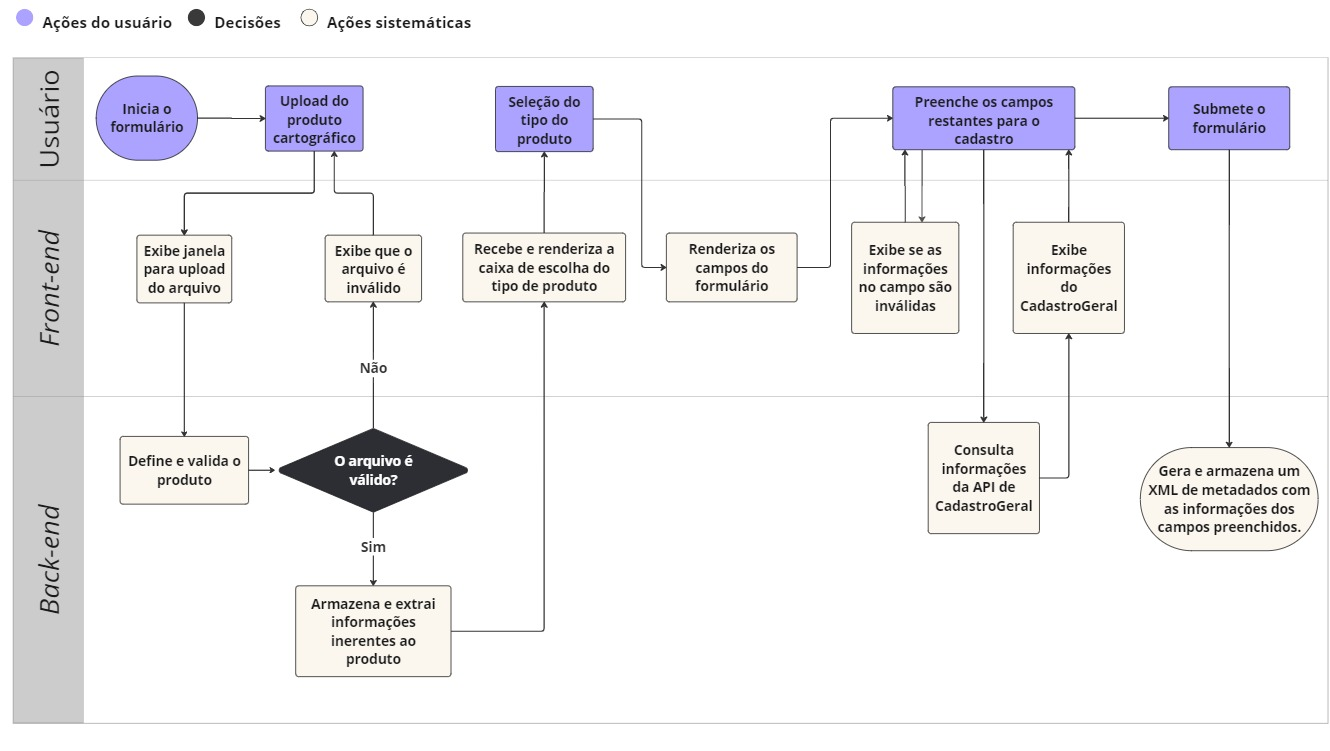
\includegraphics[width=1\linewidth]{img/fluxograma_da_solucao.jpg}
    \caption{Fluxograma principal do cadastro de metadados.}
    \label{fig:fluxograma_da_solucao} % Rótulo para referência cruzada
\end{figure}

%Aqui vai a explicação de cada caixinha.
Neste fluxo o cadastrador de metadados inicia o formulário carregando um arquivo geoespacial (Cartas topográficas, ortoimagens, Modelos digitais de superfícies, etc) por meio do \textit{front-end} que o envia para o \textit{back-end}. O \textit{back-end} valida se o arquivo é compatível com alguns tipos de produtos e define quais desses tipos de produto ele pode ser. Caso o arquivo seja inválido, o usuário recebe uma mensagem de erro e deve realizar novamente o upload de um produto, e caso o arquivo seja válido, o \textit{back-end} armazena o produto no banco de dados e extrai algumas informações de metadados do produto de forma automatizada. Caso o processamento do \textit{back-end} tenha sucesso, ele retorna ao \textit{front-end} os tipos de produto que o usuário pode cadastrar, bem como os metadados que compõe cada tipo, a id do produto armazenado e os campos que foram extraídos de forma automática. O usuário então seleciona o tipo de produto que ele está cadastrando, e a partir disso o \textit{front-end} renderiza os campos do formulário para o preenchimento. A medida que o usuário realiza o preenchimento é retornado a validação para cada campo, assim como as opções de preenchimento dos campos relacionados ao CadastroGeral diretamente da API que intermedia essa comunicação. Após o usuário finalizar o preenchimento e submeter o formulário, as informações são enviadas ao \textit{back-end} que gera o XML de metadados e associa ao produto já armazenado.

\section{Componentes}

% Esta seção pode ser modificada bastante dependendo de como são as entregas do projeto. Para a VE apresentem apenas as principais entregas que já podem ser identificadas. Nas demais avaliações, adicionem os "blocos" intemerdiários que foram construídos para chegar nestas entregas.
% Explicar as caixinhas do diagrama da visão geral.
% Comentar as decisões e explicar o motivo.


Nessa seção será abordado os componentes que constituem a aplicação do formulário de metadados, sendo aprofundados quais seus objetivos, como se deram suas construções, seus funcionamentos e como ocorre a interação entre eles.

\subsection{\textit{Front-end}}
\subsubsection{Componentes do formulário de metadados}

\subsubsection{Gerenciamento das chamadas ao \textit{back-end}}

\subsection{\textit{Back-end}}

\subsection{Algoritmo de cálculo de INOM e MI}
\label{sec:inom/mi}

Para simplificar o formulário atual e evitar os erros de cadastro de Indíce de nomenclatura e MI, foi desenvolvido essa função para extrair automaticamente essas variáveis com o tratamento do arquivo do produto geoespacial utilizando a biblioteca \textit{rasterio}.

O primeiro passo do algoritmo é criar uma relação de tamanhos (em graus) dos enquadramentos em cada escala, iniciando na escala de 1:1.000.000, seguindo para as escalas seguintes (500.000, 250.000, 100.000, 50.000, 25.000, 10.000, 5.000, 2.000 e, por fim, 1.000). Cada enquadramento possui um tamanho fixo quando representados em latitude e longitude. Os enquadramentos se iniciam na escala 1:1.000.000, com 4º de latitude e 6º de longitude, começando a partir do equador e da latitude -180, respectivamente. 

Os enquadramentos das escalas maiores são subdivisões sistemáticas do enquadramento de 1:1.000.000. Portanto, cada divisão é representada por um código. Por exemplo, na escala 1:500.000 os códigos V, X, Y ou Z são utilizados para identificar qual das quatro subdivisões do enquadramento de 1:1.000.000 são representadas no produto. O código obtido na subdivisão de cada escala será aqui designado por INOM parcial. O INOM de um produto é, portanto, composto pela concatenação de todos os INOM parciais obtidos pelas divisões inteiras, em cada escala, da latitude e longitude do ponto central do produto.

Os passos seguintes do algoritmo para determinar o valor do INOM podem ser descrito da seguinte forma:

\begin{enumerate}
    \item A escala do produto é obtida comparando a extensão do produto com as extensões previstas em cada escala. Ou seja, a escala cuja extensão prevista for o maior retângulo que ainda caiba dentro da extensão do produto é definida como escala do produto;
    \item São obtidas a latitude e longitude do ponto central do produto e posteriormente são calculadas as linhas ou colunas que o ponto central pertence, da grade do enquadramento sistemático de cada escala. Para representar as divisões do sistema UTM, as linhas e colunas são contadas à partir de 88º latitude (norte) e -180º longitude. É calculado o resto da divisão das linhas e colunas, pela quantidade de subdivisões de cada escala. A combinação do resto da longitude e da latitude é utilizada para identificar o INOM parcial de cada escala. Por exemplo, na escala 1:500.000 (V,X,Y,Z) um produto com resto 0 na latitude e resto 1 na longitude recebe o INOM parcial X.  Este procedimento é repetido da escala 1:500.000 até a escala do produto.
    \item Para cada escala, é definida uma regra para compor o índice de nomeclatura final:
    \begin{enumerate}
        \item Para a escala de 1.000.000: Utilizamos a Latitude para definir se o INOM começará por N ou por S, depois realizaremos uma divisão inteira da latitude e longitude para definir a linha e coluna da grade que o ponto central se encontra, e o restante do INOM é composto por: É adicionada uma letra do alfabeto da posição correspondente a divisão inteira da sua latitude (começando por A até a 22ª letra do alfabeto), e de acordo com a divisão inteira da longitude é acrescido ao nome o fuso UTM correspondente. Exemplo: O INOM SA-22.
        \item Para a escala de 1.500.000 em diante: A partir dessa escala, os retângulos definidos pela escala 1.000.000 são divididos em 4 ou 6 partes, e para cada uma dessas divisões são definidos os códigos de cada um dos "setores". Exemplo: Ao verificar a divisão inteira para o ponto central nas escalas 1:500.000 e 1:250.000, são acrescidas as letras V e B, compondo um INOM na escala 1:250.000 igual à SA-22-V-B.
    \end{enumerate}
    
\end{enumerate}

O INOM é utilizado para calcular o MI de cada produto. Foi obtida a lista de MIs do mapeamento sistemático à partir do WFS do BDGEx (ms:F100\_WGS84 e ms:F250\_WGS84). Estas tabelas foram introduzidas no sistema e representadas um modelo do Django chamado de \textit{IndexMap}. Desta forma, um método busca na tabela qual é o MI da escala 1:100.000 ou 1:250.000 que compõe a parte inicial do INOM do produto. No caso do produto ser de escalas maiores, o restante do INOM é adicionado ao MI. Por exemplo, um produto na escala 1:25.000 com INOM SD-21-X-B-III-2-NO utiliza o MI 1873, relativo à parte SD-21-X-B-III do INOM (da escala 1:100.000), e as subdivisões -2-NO. Assim, o MI calculado seria 1873-2-NO. 

Como o INOM é obtido pelas extensões espaciais do arquivo do produto, este procedimento permite obter também o MI. Caso o produto tenha tamanho compatível com a escala, porém não cubra o produto completamente a região, será considerado não sistemático.




\chapter{Resultados e discussão}

%Mostrar como ficou o produto final que foi planejado no capítulo anterior
%Explicar detalhes interessantes com exemplos em figuras. Principalmente, procedimentos que foram adotados para verificar se tudo funciona e ocorreu conforme o planejado. Ex.: Capturas de telas do produto funcionando nos principais casos de uso, procedimentos de testes unitários, verificação de qualidade, etc.

Neste capítulo será abordado os resultados da aplicação que foi desenvolvida a partir dos requisitos funcionais e não-funcionais descritos na seção \ref{sec:requisitos}, bem como as comparações com a aplicação atual do BDGEx.



\chapter{Conclusão}

\section{Considerações finais}

% Parágrafo curto de visão geral do que foi feito no trabalho.
% Parágrafos explicando as principais entregas do projeto (1 por entrega). Breves comentários sobre coisas interessantes de cada entrega.
% 1 Parágrafo de fechamento, geralmente contendo os impactos do projeto ou o que foi agregado com essa experiência.

Neste trabalho, foi desenvolvida uma nova aplicação web para o cadastro e validação de metadados dos produtos cartográficos da Diretoria de Serviço Geográfico do Exército Brasileiro (DSG), com o objetivo de modernizar e otimizar o processo existente no BDGEx. A solução buscou superar limitações identificadas na estrutura anterior, especialmente no que tange à integração com sistemas externos, à automação de tarefas manuais e à conformidade com normas técnicas. O projeto focou na criação de uma arquitetura desacoplada, na automação do preenchimento de dados geoespaciais, na validação eficiente de metadados e na geração automática de arquivos XML padronizados.




\section{Trabalhos futuros}

% Ver seção da EAP
%\input{exemplo-cap-01}
%\input{exemplo-cap-02}
%\input{exemplo-conclusao}

% ----------------------------------------------------------
% ELEMENTOS PÓS-TEXTUAIS
% ----------------------------------------------------------
\postextual
% ----------------------------------------------------------

% ----------------------------------------------------------
% Referências bibliográficas
% ----------------------------------------------------------
\bibliography{refs}

% ----------------------------------------------------------
% Apêndices
% ----------------------------------------------------------
\begin{apendicesenv}
    \partapendices
    %\input{exemplo-apendice}
\end{apendicesenv}
% ---

% ----------------------------------------------------------
% Anexos
% ----------------------------------------------------------
\begin{anexosenv}
    \partanexos
    %\input{exemplo-anexo}
\end{anexosenv}

%---------------------------------------------------------------------
% INDICE REMISSIVO
%---------------------------------------------------------------------
\phantompart
\printindex
%---------------------------------------------------------------------

\end{document}
